\documentclass{article}
\usepackage[utf8]{inputenc}
\usepackage{polski}
\usepackage{geometry}
\usepackage{pdfpages}
\usepackage{pdfpages}
\usepackage{listings}
\usepackage{listingsutf8}
\usepackage{multirow}
\usepackage{siunitx}
\usepackage{multirow}
\usepackage{booktabs}
\usepackage{tabularx}
\usepackage{placeins}
\usepackage{pdflscape}
\usepackage{graphicx}
\usepackage{subfig}
\usepackage{hyperref}
\usepackage{amsmath}
\usepackage{colortbl}

\geometry{
a4paper,
total={170mm,257mm},
left=20mm,
top=20mm
}
\newcolumntype{Y}{>{\centering\arraybackslash}X}
% \renewcommand\thesection{}
\lstset{%
literate=%
 {ą}{{\k{a}}}1
 {ę}{{\k{e}}}1
 {Ą}{{\k{A}}}1
 {Ę}{{\k{E}}}1
 {ś}{{\'{s}}}1
 {Ś}{{\'{S}}}1
 {ź}{{\'{z}}}1
 {Ź}{{\'{Z}}}1
 {ń}{{\'{n}}}1
 {Ń}{{\'{N}}}1
 {ć}{{\'{c}}}1
 {Ć}{{\'{C}}}1
 {ó}{{\'{o}}}1
 {Ó}{{\'{O}}}1
 {ż}{{\.{z}}}1
 {Ż}{{\.{Z}}}1
 {ł}{{\l{}}}1
 {Ł}{{\l{}}}1
}

\title{Metody Programowania Równoległego\\ Cuda - VectorAdd}
\author{Maciej Trątnowiecki}
\date{AGH, Semestr Letni, 2022}

\begin{document}
    \maketitle
    \lstset{ 
      backgroundcolor=\color{white},   % choose the background color; you must add \usepackage{color} or \usepackage{xcolor}; should come as last argument
      basicstyle=\footnotesize,        % the size of the fonts that are used for the code
      breakatwhitespace=false,         % sets if automatic breaks should only happen at whitespace
      breaklines=true,                 % sets automatic line breaking
      captionpos=b,                    % sets the caption-position to bottom
      commentstyle=\color{mygreen},    % comment style
      deletekeywords={...},            % if you want to delete keywords from the given language
      escapeinside={\%*}{*)},          % if you want to add LaTeX within your code
      %extendedchars=true,              % lets you use non-ASCII characters; for 8-bits encodings only, does not work with UTF-8
      firstnumber=1000,                % start line enumeration with line 1000
      frame=single,	                   % adds a frame around the code
      keepspaces=true,                 % keeps spaces in text, useful for keeping indentation of code (possibly needs columns=flexible)
      keywordstyle=\color{blue},       % keyword style
      language=Octave,                 % the language of the code
      morekeywords={*,...},            % if you want to add more keywords to the set
      numbers=left,                    % where to put the line-numbers; possible values are (none, left, right)
      numbersep=5pt,                   % how far the line-numbers are from the code
      numberstyle=\tiny\color{mygray}, % the style that is used for the line-numbers
      rulecolor=\color{black},         % if not set, the frame-color may be changed on line-breaks within not-black text (e.g. comments (green here))
      showspaces=false,                % show spaces everywhere adding particular underscores; it overrides 'showstringspaces'
      showstringspaces=false,          % underline spaces within strings only
      showtabs=false,                  % show tabs within strings adding particular underscores
      stepnumber=2,                    % the step between two line-numbers. If it's 1, each line will be numbered
      stringstyle=\color{mymauve},     % string literal style
      tabsize=2,	                   % sets default tabsize to 2 spaces
      title=\lstname                   % show the filename of files included with \lstinputlisting; also try caption instead of title
    }
    
    \section{Pomiary i wyniki}
        W ramach laboratorium przygotowałem odpowiednio zmodyfikowany kod programu implementującego dodawanie wektorów (opierając się na przygotowanym przez nvidię programie przykładowym) i dokonałem pomiarów czasu wykonania. Wyniki zebrałem w poniższej tabeli oraz zilustrowałem za pomocą poniższych wykresów. Analizując wykresy widzimy, że dla odpowiednio małych rozmiarów wektorów czas wykonania programu może być mniejszy bez użycia akceleracji za pomocą karty graficznej. Wynika to z narzutu czasowego generowanego przez obsługę pamięci karty graficznej i kopiowanie danych. Obserwując wykres wpływu zmiany ilości wątków na blok dla obliczeń wykonywanych z wykorzystaniem karty graficznej zauważyć możemy, że ma on ten sam kształt (w skali logarytmicznej) dla każdego rozmiaru dodawanych wektorów.
        \begin{center}
            % \begin{tabular}{lrrlrr}
            \begin{tabular}{|c|c|c|c|c|c|}
            \hline
             & elements & time & type & threads\_per\_block & blocks\_per\_grid \\
             \hline
            0 & 5000 & 0.019456 & cpu & nan & nan \\
            1 & 5000 & 1.073056 & gpu & 32.000000 & 157.000000 \\
            2 & 5000 & 0.935136 & gpu & 64.000000 & 79.000000 \\
            3 & 5000 & 0.986880 & gpu & 128.000000 & 40.000000 \\
            4 & 5000 & 0.921024 & gpu & 256.000000 & 20.000000 \\
            5 & 5000 & 1.238368 & gpu & 512.000000 & 10.000000 \\
            6 & 50000 & 0.188416 & cpu & nan & nan \\
            7 & 50000 & 1.054368 & gpu & 32.000000 & 1563.000000 \\
            8 & 50000 & 1.076416 & gpu & 32.000000 & 1563.000000 \\
            9 & 50000 & 0.995840 & gpu & 64.000000 & 782.000000 \\
            10 & 50000 & 1.157600 & gpu & 128.000000 & 391.000000 \\
            11 & 50000 & 0.990336 & gpu & 256.000000 & 196.000000 \\
            12 & 50000 & 1.080864 & gpu & 512.000000 & 98.000000 \\
            13 & 500000 & 1.808384 & cpu & nan & nan \\
            14 & 500000 & 3.273312 & gpu & 32.000000 & 15625.000000 \\
            15 & 500000 & 3.073728 & gpu & 64.000000 & 7813.000000 \\
            16 & 500000 & 3.510112 & gpu & 128.000000 & 3907.000000 \\
            17 & 500000 & 2.962688 & gpu & 256.000000 & 1954.000000 \\
            18 & 500000 & 4.000768 & gpu & 512.000000 & 977.000000 \\
            19 & 5000000 & 24.389631 & cpu & nan & nan \\
            20 & 5000000 & 12.969472 & gpu & 32.000000 & 156250.000000 \\
            21 & 5000000 & 12.517504 & gpu & 64.000000 & 78125.000000 \\
            22 & 5000000 & 13.730528 & gpu & 128.000000 & 39063.000000 \\
            23 & 5000000 & 12.097664 & gpu & 256.000000 & 19532.000000 \\
            24 & 5000000 & 12.685152 & gpu & 512.000000 & 9766.000000 \\
            25 & 10000000 & 49.402882 & cpu & nan & nan \\
            26 & 10000000 & 31.789600 & gpu & 32.000000 & 312500.000000 \\
            27 & 10000000 & 23.785185 & gpu & 64.000000 & 156250.000000 \\
            28 & 10000000 & 26.165279 & gpu & 128.000000 & 78125.000000 \\
            29 & 10000000 & 24.098751 & gpu & 256.000000 & 39063.000000 \\
            30 & 10000000 & 28.189184 & gpu & 512.000000 & 19532.000000 \\
            31 & 100000000 & 447.545349 & cpu & nan & nan \\
            32 & 100000000 & 372.130005 & gpu & 32.000000 & 3125000.000000 \\
            33 & 100000000 & 313.858063 & gpu & 64.000000 & 1562500.000000 \\
            34 & 100000000 & 229.868637 & gpu & 128.000000 & 781250.000000 \\
            35 & 100000000 & 221.865829 & gpu & 256.000000 & 390625.000000 \\
            36 & 100000000 & 234.037064 & gpu & 512.000000 & 195313.000000 \\
            \hline
            \end{tabular}
        \end{center}
        
        \begin{figure}[htb]
            \centering
            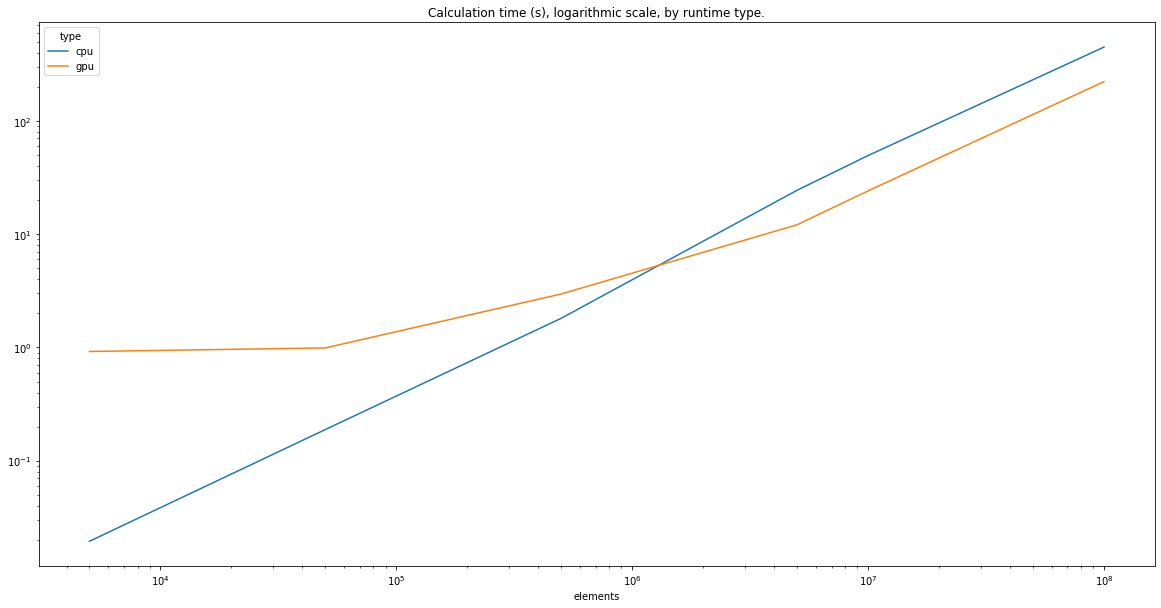
\includegraphics[width=\textwidth]{images/time_by_type.png}
            \caption{Czas wykonania programu (w sekundach) w zależności od jednostki wykonującej obliczenia, skala logarytmiczna.}
        \end{figure}
        
        \begin{figure}[htb]
            \centering
            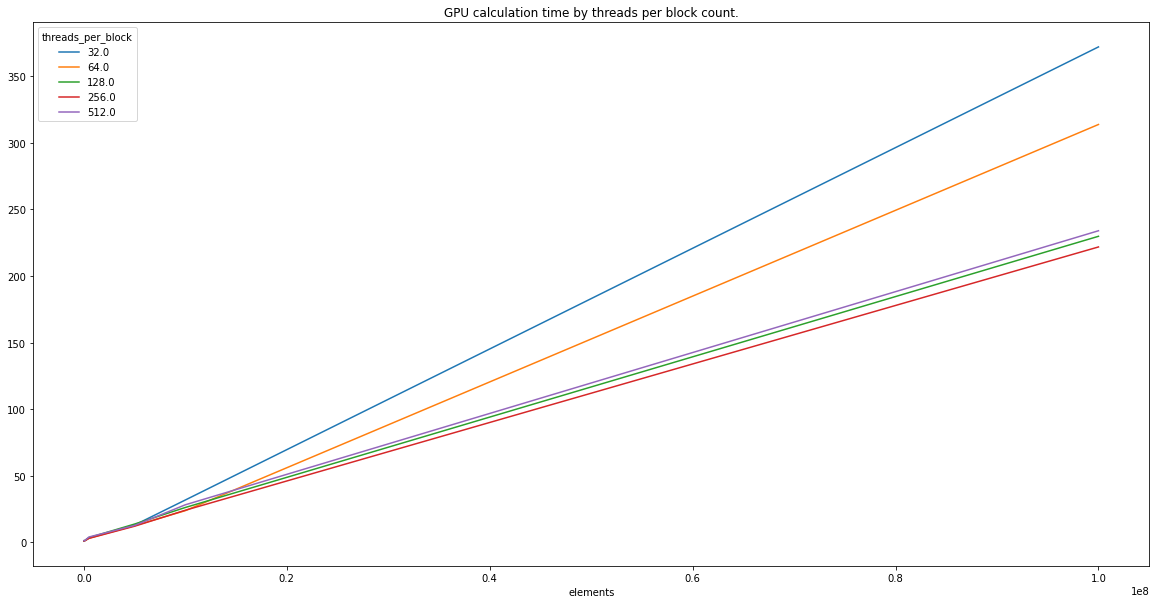
\includegraphics[width=\textwidth]{images/gpu_times.png}
            \caption{Czas wykonania programu (w sekundach) w zależności od jednostki wykonującej obliczenia, skala logarytmiczna.}
        \end{figure}

        \begin{figure}[htb]
            \centering
            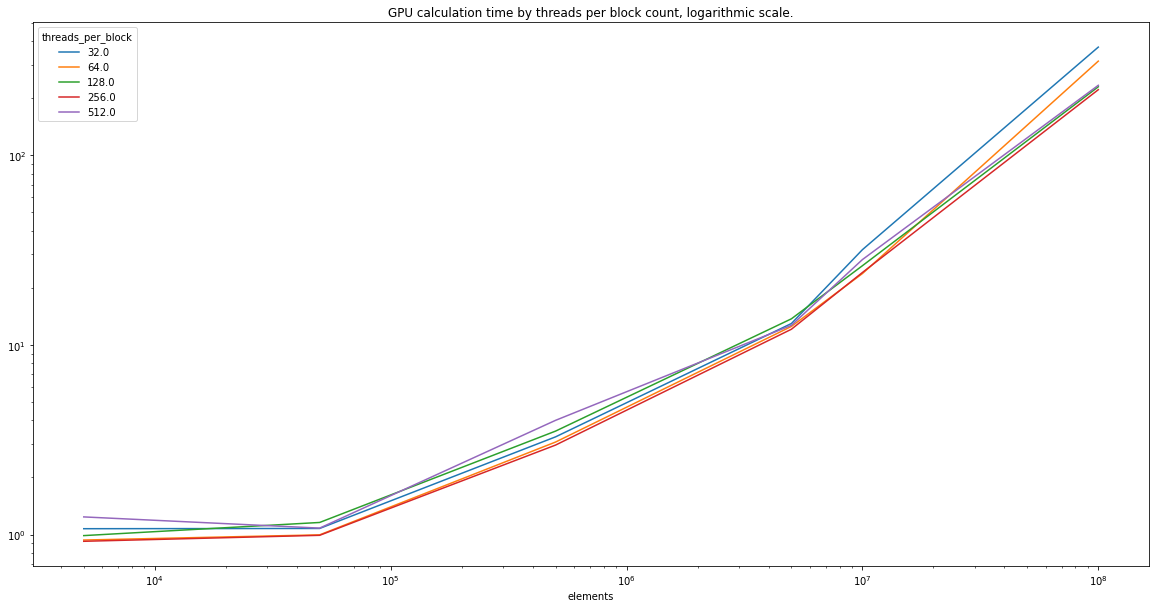
\includegraphics[width=\textwidth]{images/gpu_times_log.png}
            \caption{Czas wykonania programu (w sekundach) w zależności od jednostki wykonującej obliczenia, skala logarytmiczna.}
        \end{figure}

        \clearpage
    \section{Kod programu}
        \lstinputlisting[language=c]{../0_Simple/vectorAdd/vectorAdd.cu}
\end{document}
